\documentclass[11pt]{article}
\setlength{\parindent}{0pt}
\usepackage{xltxtra}
\usepackage{hyperref}
\hypersetup{hidelinks}
\usepackage{url}
\urlstyle{tt}
\usepackage{xcolor}
\definecolor{CVBlue}{RGB}{23,110,191}
\usepackage{calc}
\usepackage{graphicx}
\usepackage{tikz}
\usetikzlibrary{calc}
\usepackage{fontspec}
\usepackage{xeCJK}
\usepackage{enumitem}
\CJKsetecglue{} %% 取消中文与数字之间的间隙
%% 主文档字体设置
\setmainfont[
 Path = fonts/Main/,
 Extension = .otf,
 BoldFont = texgyretermes-bold.otf, % 加粗字体
]{texgyretermes-regular.otf} % 正文字体
% 中文字体设置
\setCJKmainfont[
 Path = fonts/hansans/,
 Extension = .ttf,
 BoldFont = NotoSansSC-Bold.ttf, % 加粗字体
]{NotoSansSC-Regular.ttf} % 正文字体
\usepackage{relsize}
\usepackage{xspace}
% 使用 fontawesome（部分图标）
\usepackage{fontawesome}
% A4纸，上下左右边距
\usepackage[
 a4paper,
 left=1.2cm,
 right=1.2cm,
 top=1.5cm,
 bottom=1cm,
 nohead
]{geometry}
\renewcommand{\baselinestretch}{1.5} % 行间距设为1.5
\usepackage{titlesec}
\usepackage{enumitem}
\setlist{noitemsep} % 取消列表项间的额外间距
%\setlist{nosep} % 取消所有垂直间距
\setlist[itemize]{topsep=0.25em, leftmargin=*}
\setlist[enumerate]{topsep=0.25em, leftmargin=*}
% --- 用于控制【不同项目之间】的垂直距离 ---
\newlength{\interProjectSpacing}
\setlength{\interProjectSpacing}{0.9em} % <--- 在此调整项目之间的距离
\newcommand{\projectsep}{\vspace{\interProjectSpacing}}
% --- 用于控制【项目标题】与下方【项目描述】的距离 ---
\newlength{\intraProjectTitleSep}
\setlength{\intraProjectTitleSep}{0.4em} % <--- 在此调整标题和描述的距离
\newcommand{\titlebreak}{\\[\intraProjectTitleSep]}
% --- 用于控制【项目描述】与下方【要点列表】的距离 ---
\newlength{\intraProjectListTopSep}
\setlength{\intraProjectListTopSep}{0.2em} % <--- 在此调整描述和列表的距离
% =======================================================================
\titleformat{\section} % 定制 \section 命令
 {\large\bfseries\raggedright} % 将 section 标题设置为大号、粗体且左对齐
 {}{0em} % 可用于为所有 section 添加前缀（如"章节..."）
 {} % 可用于在标题前插入代码
 [{\color{CVBlue}\titlerule}] % 在标题后插入一条横线
\titlespacing*{\section}{0cm}{*1.6}{*1.2}
\begin{document}
\pagenumbering{gobble}
%%%% 利用tikz来定位照片
% 【注意】：请将`avatar.jpg`替换为您的证件照文件名，并确保图片文件与.tex文件在同一目录，或在`\includegraphics`中指定正确路径。
% 如果您不需要照片，请删除以下\tikzpicture环境。
\begin{tikzpicture}[remember picture, overlay]
\node[anchor = north east] at ($(current page.north east)+(-2cm,-0.7cm)$) {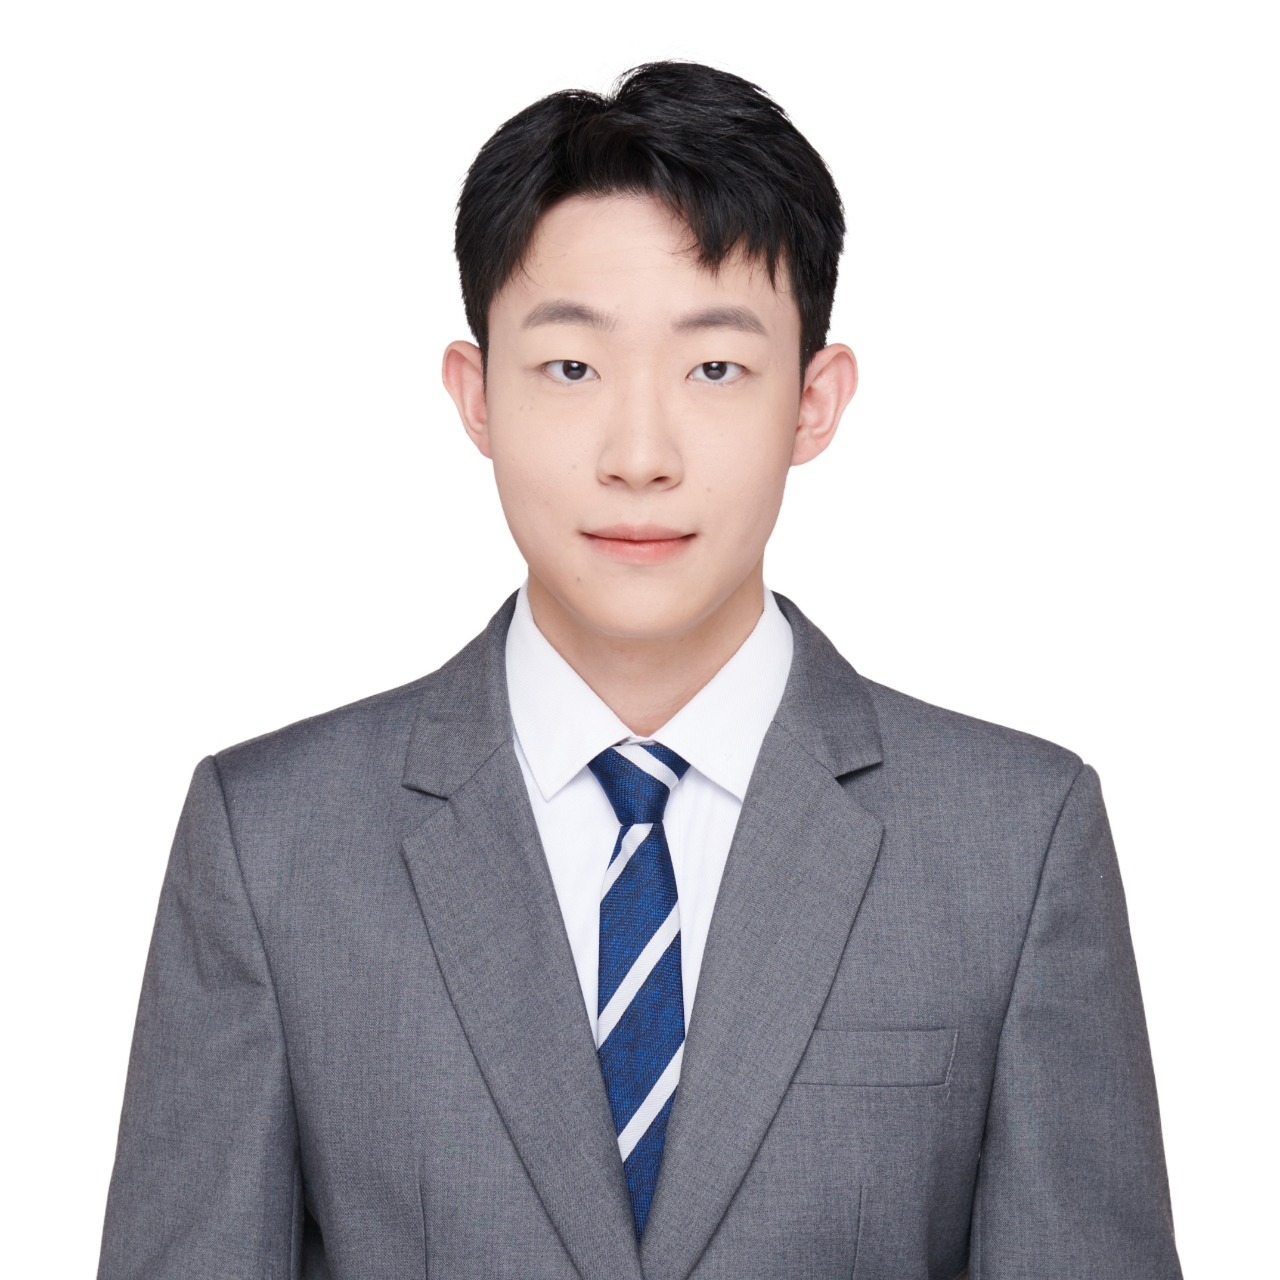
\includegraphics[height=3cm]{xu.jpg}};
\end{tikzpicture}%
%%%% 利用tikz来定位学校Logo，这里只在第一页显示
% 【注意】：请将`your_university_logo.png`替换为您学校的Logo文件名，或删除本行以移除Logo。
% 已根据您的要求，在"教育背景"部分加入了浙江大学的信息。您可以在此处使用浙江大学的Logo文件，例如 `zju-logo.png`。
\begin{tikzpicture}[remember picture, overlay]
\node[anchor = north west] at ($(current page.north west)+(0.5cm,+1.0cm)$) {\includegraphics[height=1.5cm]{zju.png}}; % 请确保图片文件存在
\end{tikzpicture}%
\centerline{\LARGE\bfseries{徐晗洋}}
\centerline{\normalsize{\faPhone\ 13915917895 \quad \faEnvelopeO\ \href{mailto:hanyangxucs@gmail.com}{hanyangxucs@gmail.com}\quad 随时到岗}}
\section{\makebox[\widthof{\faGraduationCap}][c]{\color{CVBlue}\faGraduationCap}\ 教育背景}
% ========== 浙江大学教育经历 (已补充导师信息) ==========
\textbf{浙江大学 (Zhejiang University)} \hfill 2025.9 -- 至今\\[0.5em]
计算机科学与技术 专业 \quad 硕士（保研，预计2028年毕业）
\begin{itemize}[nosep]
    \item \textbf{导师：吴健 教授}（长江学者，浙江大学求是特聘教授） % 补充导师信息
    \item \textbf{研究方向：} 多模态大模型
    \item \textbf{相关课程：} 深度学习，自然语言处理，计算机视觉
\end{itemize}
\vspace{0.5em} % 增加一点两段经历之间的间距
% ========== 电子科技大学教育经历 ==========
\textbf{电子科技大学 (University of Electronic Science and Technology of China)} \hfill 2021.9 -- 2025.6\\[0.5em]
人工智能专业 \quad 本科
\begin{itemize}[nosep]
\item \textbf{GPA: 3.97/4.0}，专业排名：5/65
\item 相关课程：数据结构与算法、机器学习、深度学习、计算机视觉、自然语言处理、概率论与数理统计
\end{itemize}
\renewcommand{\baselinestretch}{1.12}\selectfont
\section{\makebox[\widthof{\faUsers}][c]{\color{CVBlue}\faUsers}\ 研究成果与论文发表}
\textbf{npj Digital Medicine（中科院一区Top，第一作者，小修已修回）}\quad Expert-Comparable and Modality-Flexible Vision-Language Diagnosis of Non-Infectious Posterior Uveitis
\begin{itemize}[nosep]
\item \textbf{主要贡献：} 主导研究与实验设计、代码实现、全部实验开展及论文撰写。
\item \textbf{研究内容与成果：} 构建面向非感染性后葡萄膜炎诊断的多模态视觉语言框架AdaPUV，基于Qwen3-VL-8B-Instruct进行LoRA微调，融合FFA、OCT、Optos与临床文本，并系统评估缺失模态下的诊断能力。在1,834例样本队列上采用患者级独立划分，内部测试准确率达96.28\%、AUROC达0.9893；外部FFA+OCT验证准确率达94.52\%，缺少FFA时仍达92.02\%。在95例盲法阅片研究中，诊断准确率不劣于三位高年资专家。
\end{itemize}
\projectsep
\textbf{BMVC 2026（CCFC，共一，排名第二，Accepted）}\quad Beyond Classification: Structured Supervision Aligns Visual Evidence with Medical Semantics
\begin{itemize}[nosep]
\item \textbf{主要贡献：} 参与实验设计、代码实现与论文撰写。
\item \textbf{研究内容与成果：} 将ViT的背景捷径与空间对齐问题引入医学图像分类研究，在乳腺超声、皮肤镜和胸部X光三个数据集上验证高分类准确率并不保证病灶证据对齐，系统比较图自监督、分类与分割联合训练及图文对齐。相较普通ViT，图文模型微调后的平均PIB从16.8\%提升至41.0\%，揭示不同监督方式对病灶证据对齐的影响。
\end{itemize}

\section{\makebox[\widthof{\faCogs}][c]{\color{CVBlue}\faCogs}\ 技能与专长}
\begin{itemize}[nosep]
\item \textbf{英语能力：} CET-6 (627分)，具备流畅的英文技术文献阅读能力
\item \textbf{编程语言：} Python, C/C++
\item \textbf{深度学习框架：} PyTorch，TensorFlow，熟悉模型构建、训练与部署。
\end{itemize}
\section{\makebox[\widthof{\faGraduationCap}][c]{\color{CVBlue}\faList}\ 获奖情况}
\begin{itemize}[nosep]
\item 全国大学生数学竞赛（非数学类）\textbf{省级一等奖} \hfill 2023
\item 电子科技大学校级"优秀学生"\textbf{奖学金}（连续两年） \hfill 2022, 2023
\end{itemize}

\end{document}
